\documentclass[12pt]{beamer}
\usepackage[frenchb]{babel}
\usepackage[T1]{fontenc}
\usepackage[utf8x]{inputenc} 
\usepackage{ucs}   
\usepackage{graphicx}           % pictures
\usepackage{multimedia}         % sounds and movies
\usetheme{Warsaw}
\title {Projet Picross}
\author{Groupe B}
\date{16 Mai 2014}
\institute{Université du Maine}
%%%%%%%%%%%%%%%%%
% PREAMBULE     %
%%%%%%%%%%%%%%%%%
\setbeamertemplate{itemize item}[circle]
\hypersetup{
        pdfpagemode = FullScreen,% afficher le pdf en plein Ecran
        pdfauthor   = {groupe B},%
        pdftitle    = {projet}%
        pdfsubject  = {projet},%
        pdfcreator  = {PDFLaTeX},%
}
\setbeamertemplate{navigation symbols}{
        %\insertslidenavigationsymbol
        %\insertframenavigationsymbol
        %\insertsubsectionnavigationsymbol
        %\insertsectionnavigationsymbol
        %\insertdocnavigationsymbol
        %\insertbackfindforwardnavigationsymbol
}
% Faire apparaitre un sommaire avant chaque section
\AtBeginSection[]{
        \begin{frame}
        \begin{center}{\Large Plan }\end{center}
        %%% affiche en début de chaque section, les noms de sections et
        %%% noms de sous-sections de la section en cours.
        \tableofcontents[currentsection,hideothersubsections]
        \end{frame} 
}
%%%%%%%%%%%%%%%%%
% DOCUMENT      %
%%%%%%%%%%%%%%%%%
\begin{document}
\maketitle
% FRAME %%%%%%%%%%%%%%%%%%%%%%%%%%%%
\begin{frame}{}
  \tableofcontents
\end{frame}
   
%%%%%%%%%%%%%%%%%%
% Présentation
%%%%%%%%%%%%%%%%%%
\section{Présentation}
% FRAME %%%%%%%%%%%%%%%%%%%%%%%%%%%%
\begin{frame}
\frametitle{Présentation du Projet}
    \begin{enumerate}
     
      \item Présentation des membres
        \begin{itemize}
            \item Lucas Bourneuf   (Chef de Projet)
            \item Ewen Cousin      (Développeur GUI)
            \item Jaweed Parwany   (Développeur Systéme)
            \item Charlie Maréchal (Documentaliste)
            \item Nicolas Bourdin  (Développeur GUI)
            \item Julien Le Gall   (Développeur IA)
        \end{itemize}
     
      \item Objectif
        \begin{itemize}
            \item Créer un Picross en Ruby
        \end{itemize}
     
      \item Delai
        \begin{itemize}
            \item 3 mois
        \end{itemize}
 \end{enumerate}   
 \end{frame}
    
   \begin{frame}
   \begin{enumerate}
   \item Liste des fonctionnalités
    
    \begin{itemize}
        \item Gestion de sauvegarde
        \item Drag 'n' Assign
        \item Score
        \item Aide
        \item Édition
        \item Manuels
    \end{itemize}
    
    
    \pause
    \item Contraintes 
    \begin{enumerate}
        \item Temps
        \item Technique
    \end{enumerate}
    
    %\item "Il s'agit d'un picross blablabla"
    
    \end{enumerate}
\end{frame}


\section{Réalisation du projet}
\subsection{Le déroulement du projet}


\begin{frame}
  \frametitle{Diagramme de Gantt}
  \begin{figure}[t]
    \centering
    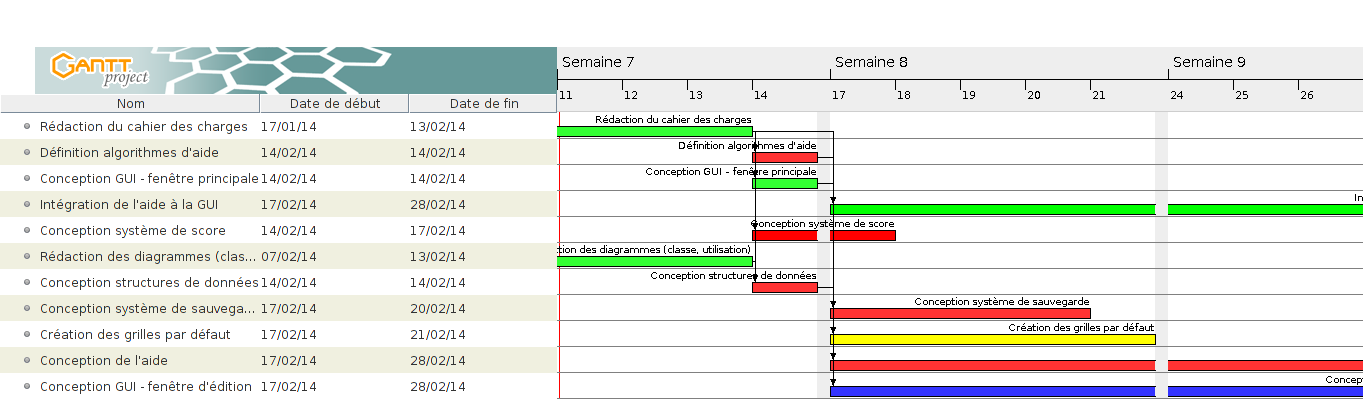
\includegraphics[scale=0.38]{data/ganttDiagram}
    \caption{Diagramme de Gantt}
  \end{figure}
\end{frame}


\begin{frame}
  \frametitle{Diagramme UML Système}
  \begin{figure}
    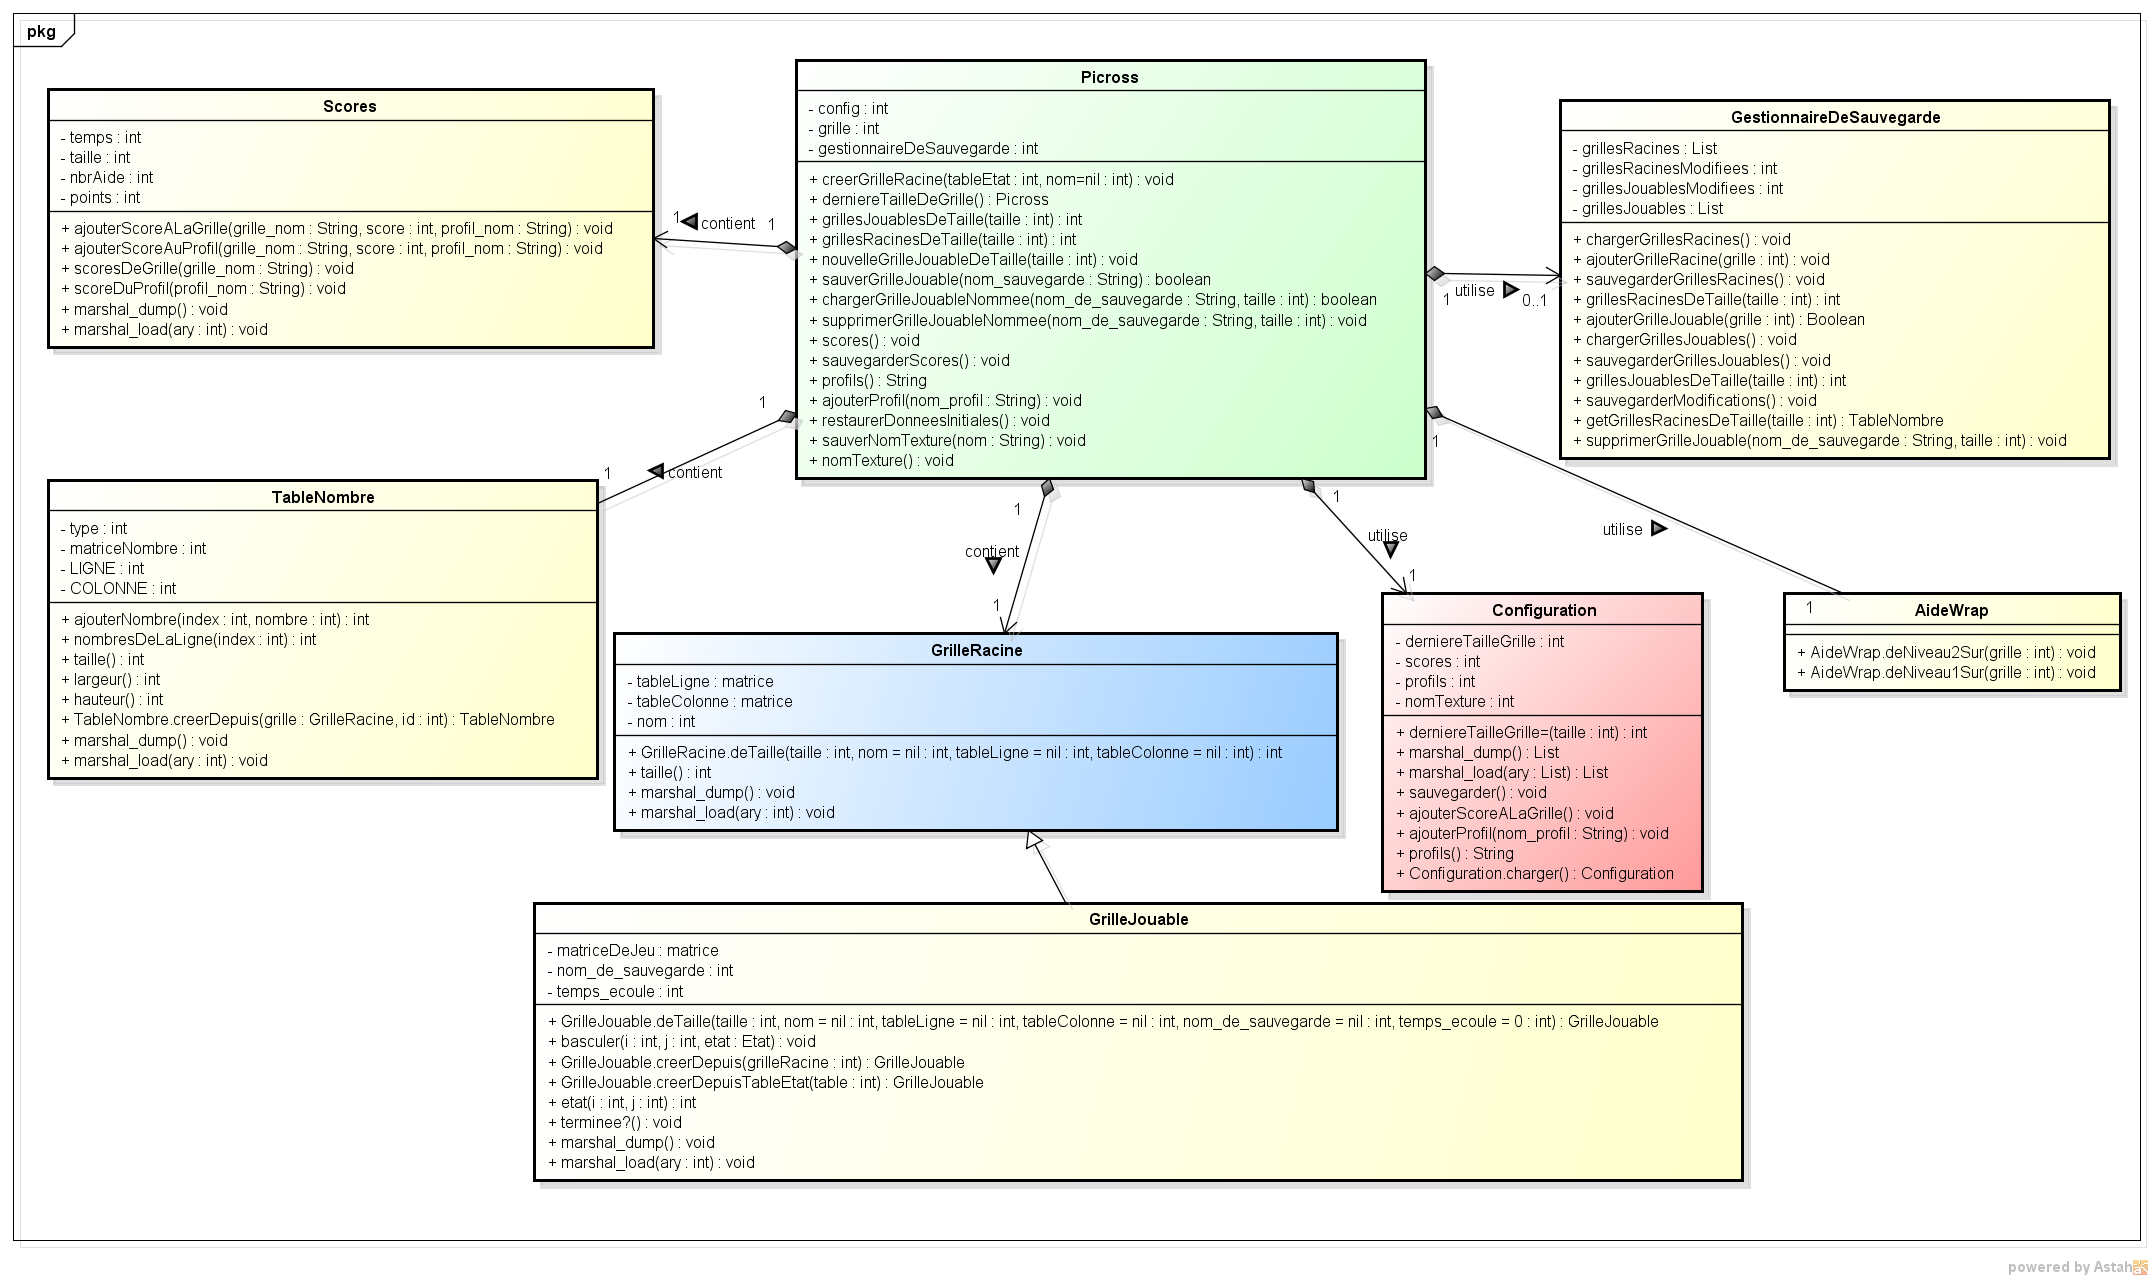
\includegraphics[scale=0.20]{data/UMLDiagram}
    \caption{Diagramme UML Système}
  \end{figure}
\end{frame}

\begin{frame}
  \frametitle{Diagramme UML GUI}
  \begin{figure}
    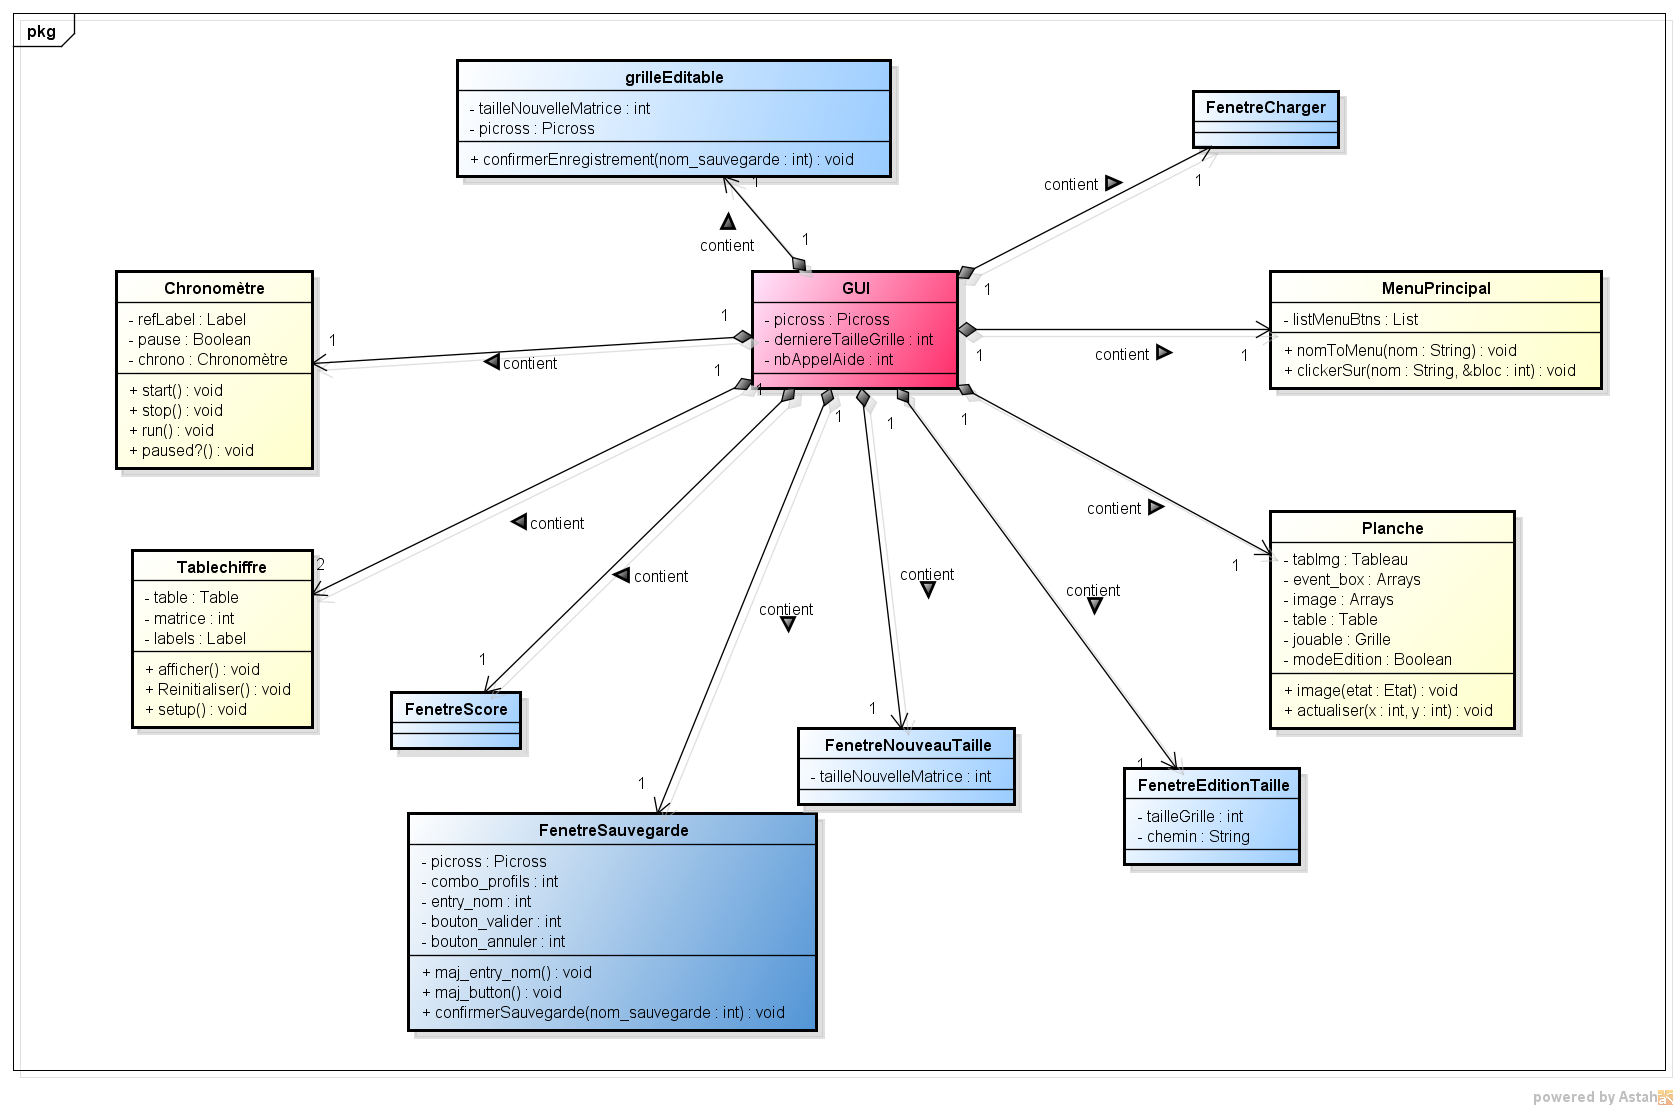
\includegraphics[scale=0.23]{data/UMLGUI}
    \caption{Diagramme UML GUI}
  \end{figure}
\end{frame}

\subsection{Aspects techniques}
    \begin{frame}
    \frametitle{Aspects techniques}
    
        \begin{itemize}
            \item Languages
            \pause
            \item Support
            \pause
            \item Outils
            \begin{itemize}
                \item IDE,
                \item Modules ruby,
                \item IRC,
                \item Etherpad,
                \item Git/Github,
                \item GanttProject,
                \item Astah;
            \end{itemize}
                    
        \end{itemize}
\end{frame}

\subsection{Partage des tâches}
    \begin{frame}
    \frametitle{Partage des tâches}
        \begin{itemize}
            \item Système : Lucas Bourneuf, Charlie Maréchal, Jaweed Parwany
            \smallskip
            \smallskip
            \item GUI : Ewen Cousin, Nicolas Bourdin
            \smallskip
            \smallskip
            \item Aide : Julien Le Gall
        \end{itemize}
    \end{frame}


\subsection{Difficultés}
    \begin{frame}
    \frametitle{Difficultés}
        \begin{itemize}
          \item Travailler en groupe;
          \smallskip
          \smallskip
          \item répartition des tâches;
          \smallskip
          \smallskip
          \item utilisation de git.
        \end{itemize}
    \end{frame}

\section{Démonstration}
    \begin{frame}{Démonstration}
    \end{frame}

\section{Conclusion}
    \begin{frame}
    \frametitle{Conclusion}
        
        \begin{enumerate}
            \item Perspectives d'améliorations
            \begin{itemize}
                \item Statistiques d'un profil;
                \item amélioration de l'interface.
            \end{itemize}
            
            \pause
            \item Ce que l'on a appris
            \begin{enumerate}
                \item Comment un projet se déroule;
                \item le travail collaboratif.
            \end{enumerate}
            
            \pause
            \item Ce que l'on a aimé;
            
         
        \end{enumerate}
    \end{frame}
    
    \begin{frame}
    \frametitle{Conclusion}
        {\Huge Questions ?}
    \end{frame}
\end{document}
